% =============================================================================
% Proxy SOCKS5 - Trabajo Práctico Especial
% Protocolos de Comunicación - ITBA - 2026
% =============================================================================
\documentclass[12pt,a4paper]{article}

% ---- Paquetes ----
\usepackage[utf8]{inputenc}
\usepackage{lmodern}
\usepackage[T1]{fontenc}
\usepackage[spanish]{babel}
\usepackage{geometry}
\geometry{left=2.5cm,right=2.5cm,top=2.5cm,bottom=2.5cm}
\usepackage{hyperref}
\usepackage{listings}
\usepackage{xcolor}
\usepackage{graphicx}
\usepackage{enumitem}
\usepackage{float}
\usepackage{fancyhdr}
\setlength{\headheight}{15pt}
\usepackage{titlesec}
\usepackage{booktabs}
\usepackage{verbatim}

% ---- Configuración de listings ----
\lstset{
    basicstyle=\ttfamily\small,
    breaklines=true,
    frame=single,
    numbers=left,
    numberstyle=\tiny,
    backgroundcolor=\color{gray!10},
    rulecolor=\color{gray!30},
    captionpos=b,
    tabsize=4,
    showstringspaces=false,
    language=C,
    keywordstyle=\color{blue},
    stringstyle=\color{red},
    commentstyle=\color{green!50!black},
    literate=
        {á}{{\'a}}1 {é}{{\'e}}1 {í}{{\'i}}1 {ó}{{\'o}}1 {ú}{{\'u}}1
        {Á}{{\'A}}1 {É}{{\'E}}1 {Í}{{\'I}}1 {Ó}{{\'O}}1 {Ú}{{\'U}}1
        {ñ}{{\~n}}1 {Ñ}{{\~N}}1 {ü}{{\"u}}1 {Ü}{{\"U}}1
        {¿}{{?`}}1 {¡}{{!`}}1
}

% ---- Configuración de encabezados ----
\pagestyle{fancy}
\fancyhf{}
\fancyhead[L]{Proxy SOCKS5}
\fancyhead[R]{Protocolos de Comunicación --- 2026}
\fancyfoot[C]{\thepage}

% ---- Redefinir títulos de secciones ----
\titleformat{\section}{\Large\bfseries}{\thesection}{1em}{}
\titleformat{\subsection}{\large\bfseries}{\thesubsection}{1em}{}

% ---- Portada ----
\title{\textbf{Trabajo Práctico Especial}\\[1cm]
       
\includegraphics[width=0.5\textwidth]{scripts/results/itba.png}\\[1cm]
       \Large{Proxy SOCKS5}\\[0.3cm]
       \large{Protocolos de Comunicación 2026}}

\author{\textbf{Grupo 2}\\[0.3cm]
        Tiago Heras - 65627 \\[0.1cm]
        Mateo Arias - 65613\\[0.1cm]
        Amador Vallejo Tapia - 65454\\[0.1cm]
        Manuel García Puente - 65505\\[8cm]
        \textbf{Instituto Tecnológico de Buenos Aires}}
\date{14 de julio de 2026}

\begin{document}

\maketitle
\thispagestyle{empty}
\newpage

% =============================================================================
\tableofcontents
\newpage

% =============================================================================
\section{Descripción detallada de los protocolos diseñados y aplicaciones desarrolladas}

\subsection{Arquitectura general del servidor proxy SOCKS5}

El servidor proxy SOCKS5 está implementado como una aplicación monohilo que utiliza
multiplexación de entrada/salida no bloqueante mediante un selector de eventos.
Todas las conexiones entrantes y salientes se manejan en un único hilo de ejecución,
con la única excepción de la resolución de nombres de dominio (FQDN), que se delega
a un hilo auxiliar mediante \texttt{getaddrinfo(3)}.

Cada conexión SOCKS5 se modela como una máquina de estados que transiciona a través
de las siguientes fases:

\begin{verbatim}
HELLO_READ -> HELLO_WRITE -> [AUTH_READ -> AUTH_WRITE] -> REQUEST_READ
    -> REQUEST_RESOLV -> REQUEST_CONNECTING -> REQUEST_WRITE -> COPY
    -> DONE / ERROR
\end{verbatim}

\begin{itemize}
    \item \textbf{HELLO}: el cliente ofrece métodos de autenticación; el servidor
          elige \texttt{NO AUTH} si no hay usuarios registrados, o usuario/contraseña
          (RFC~1929) en caso contrario.
    \item \textbf{AUTH}: si corresponde, se validan las credenciales contra la tabla
          en memoria (hasta 10 usuarios, configurables por CLI o en caliente).
    \item \textbf{REQUEST}: solo se soporta \texttt{CONNECT}. Se aceptan destinos
          IPv4, IPv6 y FQDN. Si un FQDN resuelve a varias direcciones, se intentan
          en orden hasta lograr conectar.
    \item \textbf{COPY}: túnel bidireccional. Tras cada lectura exitosa se intenta
          un \texttt{write} inmediato al peer (\texttt{select $\rightarrow$ read
          $\rightarrow$ write}); si no entra todo, el resto queda en el buffer y se
          espera \texttt{OP\_WRITE}.
\end{itemize}

\subsection{Protocolo de monitoreo y configuración}

\subsubsection{Descripción general}

El protocolo de monitoreo es un protocolo de texto sobre TCP, independiente de SOCKS5,
expuesto en un socket pasivo propio (por defecto \texttt{127.0.0.1:8080}). Permite
consultar métricas y modificar usuarios o el secreto de administración sin reiniciar
el servidor.

\subsubsection{Decisiones de diseño}

\begin{itemize}
    \item \textbf{Texto plano}: facilita depuración y una especificación estilo RFC
          sin serialización binaria.
    \item \textbf{Una línea por comando / una línea por respuesta}: el estado por
          conexión es mínimo y encaja en la misma STM del selector.
    \item \textbf{Autenticación por secreto compartido}: cada comando comienza con
          un token secreto configurado con \texttt{-A} (y cambiable en runtime con
          \texttt{SET\_SECRET}). Sin el secreto correcto, la respuesta es
          \texttt{-ERR unauthorized}.
    \item \textbf{Terminadores}: los comandos aceptan \texttt{LF} o \texttt{CRLF}
          (el \texttt{CR} opcional se ignora). Las respuestas siempre se emiten con
          \texttt{CRLF}. Se eligió esta asimetría a propósito: ser permisivos al
          parsear (compatible con clientes que mandan solo \texttt{\textbackslash n})
          y estrictos al responder (línea bien formada para parsers que esperan
          \texttt{CRLF}).
\end{itemize}

\subsubsection{Formato de los mensajes}

\begin{lstlisting}[caption=Gramática ABNF de comandos]
comando     = secreto SP verbo *(SP argumento) EOL
secreto     = 1*(%x21-7E)
verbo       = 1*ALPHA
argumento   = 1*(%x21-7E)
EOL         = [CR] LF
CR          = %x0D
LF          = %x0A
SP          = %x20
\end{lstlisting}

\begin{lstlisting}[caption=Gramática ABNF de respuestas]
respuesta   = status [SP datos] CRLF
status      = "+OK" / "-ERR"
datos       = 1*(%x20-7E)
CRLF        = CR LF
\end{lstlisting}

\subsubsection{Comandos soportados}

\begin{enumerate}
    \item \textbf{GET\_METRICS}
    \begin{itemize}
        \item Sintaxis: \texttt{<secreto> GET\_METRICS\textbackslash n}
        \item El cliente imprime tres líneas con las métricas obtenidas:
              \texttt{conexiones activas: <n>}, \texttt{conexiones historicas: <n>},
              \texttt{bytes transferidos: <n>}.
        \item \texttt{ACT}: conexiones SOCKS5 activas (ya aceptadas y en curso).
        \item \texttt{HIST}: conexiones históricas desde el arranque.
        \item \texttt{BYTES}: bytes transferidos en el túnel (ambos sentidos).
    \end{itemize}

    \item \textbf{ADD\_USER}
    \begin{itemize}
        \item Sintaxis: \texttt{<secreto> ADD\_USER <usuario> <contraseña>\textbackslash n}
        \item Hay un espacio entre el usuario y la contraseña.
        \item En caso de éxito el cliente imprime \texttt{usuario agregado}.
        \item En caso de error el cliente imprime \texttt{error: <motivo>} por stderr.
        \item Máximo 10 usuarios; cada campo hasta 255 caracteres.
    \end{itemize}

    \item \textbf{DEL\_USER}
    \begin{itemize}
        \item Sintaxis: \texttt{<secreto> DEL\_USER <usuario>\textbackslash n}
        \item En caso de éxito el cliente imprime \texttt{usuario eliminado}.
        \item En caso de error el cliente imprime \texttt{error: user not found} por stderr.
    \end{itemize}

    \item \textbf{SET\_SECRET}
    \begin{itemize}
        \item Sintaxis: \texttt{<secreto> SET\_SECRET <nuevo\_secreto>\textbackslash n}
        \item Cambia el secreto de management en caliente.
        \item En caso de éxito el cliente imprime \texttt{secreto actualizado}.
    \end{itemize}
\end{enumerate}

\subsubsection{Flujo de una sesión típica}

A continuación se muestra un ejemplo de una sesión de monitoreo utilizando el
cliente provisto. Nótese que el cliente traduce internamente las respuestas del
protocolo (\texttt{+OK ...\textbackslash r\textbackslash n}) a mensajes legibles
para el usuario; no se vuelca el formato de red a la consola.

\begin{lstlisting}[caption=Ejemplo de sesión de monitoreo con el cliente]
$ ./bin/client -A changeme get-metrics
conexiones activas: 3
conexiones historicas: 150
bytes transferidos: 1048576

$ ./bin/client -A changeme add-user alberto pass123
usuario agregado

$ ./bin/client -A changeme del-user alberto
usuario eliminado
\end{lstlisting}

El protocolo subyacente intercambia las siguientes líneas (no visibles para el
usuario del cliente):

\begin{lstlisting}[caption=Formato de red subyacente (wire format)]
>> changeme GET_METRICS\n
<< +OK ACT:3 HIST:150 BYTES:1048576\r\n
>> changeme ADD_USER alberto pass123\n
<< +OK\r\n
>> changeme DEL_USER alberto\n
<< +OK\r\n
\end{lstlisting}

\subsection{Aplicación cliente de monitoreo}

El cliente es una CLI con I/O bloqueante que abstrae el protocolo: arma el comando
con el secreto (\texttt{-A}), envía una línea, lee la respuesta hasta \texttt{CRLF}
y presenta un mensaje legible. No vuelca el wire format a stdout.

\begin{lstlisting}[caption=Uso del cliente de monitoreo]
./bin/client [opciones] <comando>

Opciones:
  -L <dirección>   IP del servidor de management (defecto: 127.0.0.1)
  -P <puerto>      Puerto de management (defecto: 8080)
  -A <secreto>     Secreto de management (defecto: changeme)

Comandos:
  get-metrics
  add-user <usr> <pass>
  del-user <usr>
  set-secret <nuevo_secreto>
\end{lstlisting}

\begin{lstlisting}[caption=Ejemplos del cliente]
$ ./bin/client -A changeme get-metrics
conexiones activas: 0
conexiones historicas: 12
bytes transferidos: 409600

$ ./bin/client -A changeme add-user juan pass123
usuario agregado
\end{lstlisting}

Ante \texttt{-ERR} o fallo de red, el proceso termina con código de salida distinto de 0.

\subsection{Métricas y registro de accesos}

Las métricas \texttt{ACT}, \texttt{HIST} y \texttt{BYTES} son volátiles (se pierden
al reiniciar). Los accesos exitosos al origen se registran en \textbf{stdout} con
formato:

\begin{verbatim}
[YYYY-MM-DD HH:MM:SS] User: <usr> | FQDN: <nombre|-> | IP Destino: <ip:port>
\end{verbatim}

El administrador puede redirigir la salida del servidor a un archivo
(\texttt{./bin/server ... > access.log}).

% =============================================================================
\section{Problemas encontrados durante el diseño y la implementación}

\begin{itemize}
    \item \textbf{Resolución DNS no bloqueante}: \texttt{getaddrinfo(3)} bloquea.
          Se ejecuta en un hilo auxiliar y se notifica al selector con
          \texttt{selector\_notify\_block}. Hubo que cuidar el ciclo de vida del
          \texttt{struct socks5} (no liberarlo mientras el hilo DNS aún corre) y
          el acceso a \texttt{origin\_resolution}.
    \item \textbf{Múltiples direcciones por FQDN}: si la primera IP falla, hay que
          recorrer el resto de \texttt{addrinfo} sin perder el estado de la STM ni
          dejar fds huérfanos.
    \item \textbf{Graceful shutdown}: ante \texttt{SIGTERM}/\texttt{SIGINT} se deja
          de aceptar conexiones nuevas y se espera a que las activas terminen. El
          desafío fue coordinar el socket pasivo (dejar de escucharlo) con el
          contador de conexiones vivas sin cortar túneles en COPY.
    \item \textbf{Latencia extra en el túnel}: el patrón inicial
          \texttt{select $\rightarrow$ read $\rightarrow$ select $\rightarrow$ write}
          introducía un round-trip de selector innecesario. Se corrigió con write
          optimista inmediato tras cada lectura exitosa.
    \item \textbf{Autenticación dinámica}: pasar de ``sin usuarios = NO AUTH'' a
          ``hay usuarios = exigir RFC~1929'' en caliente (vía \texttt{ADD\_USER})
          obliga a que la selección de método HELLO consulte el estado actual de
          la tabla, no una política fija de arranque.
\end{itemize}

% =============================================================================
\section{Limitaciones de la aplicación}

\subsection{Capacidad del selector y file descriptors}

El selector se crea con capacidad fija (1024 descriptores). Cada túnel SOCKS usa
dos fds (cliente y origen). En pruebas de estrés, 500 conexiones concurrentes se
establecen correctamente; por encima de ese orden (p.ej.\ 750) aparecen fallos por
agotamiento de capacidad del multiplexor, no por el \textit{backlog} de
\texttt{listen(2)}.

\subsection{Backlog de \texttt{listen} vs.\ clientes conectados}

El socket pasivo usa \texttt{listen(server, SOMAXCONN)}. Ese backlog es la cola de
conexiones \textbf{pendientes de \texttt{accept}}, no el número de clientes ya
conectados. La cantidad de clientes concurrentes reales se refleja en la métrica
\texttt{ACT} (conexiones SOCKS5 activas). Confundir ambos conceptos lleva a
subestimar o sobrestimar la capacidad del servidor.

\subsection{Registro de accesos síncrono}

Los logs van a stdout con I/O bloqueante. En localhost el impacto es bajo; bajo
carga alta con un filesystem lento podría introducir micro-pausas en el event loop.
Un logger asíncrono sería una extensión natural.

\subsection{Alcance del protocolo SOCKS}

Solo se implementa \texttt{CONNECT}. No hay \texttt{BIND} ni \texttt{UDP ASSOCIATE}.
El management escucha solo en IPv4 (\texttt{AF\_INET}).

% =============================================================================
\section{Posibles extensiones}

\begin{itemize}
    \item \textbf{Dissector de credenciales (segunda entrega)}: inspección en COPY
          de protocolos en texto claro (POP3 como mínimo), estilo ettercap.
    \item \textbf{Soporte BIND y UDP ASSOCIATE}.
    \item \textbf{Logging asincrónico}: buffer en memoria y volcado diferido.
    \item \textbf{Configuración dinámica extendida}: timeouts, tamaño de buffers,
          tope de conexiones concurrentes.
    \item \textbf{Management dual-stack}: escuchar también en IPv6.
    \item \textbf{Estadísticas avanzadas}: latencia, throughput por usuario, etc.
\end{itemize}

% =============================================================================
\section{Conclusiones}

El desarrollo de este trabajo práctico permitió consolidar los conocimientos teóricos 
adquiridos a lo largo del cuatrimestre. A través de la implementación del servidor 
proxy SOCKS5, se lograron afianzar conceptos como la comunicación entre clientes y 
servidores, el funcionamiento de los protocolos de aplicación y transporte, y la 
programación avanzada con sockets activos y pasivos empleando selectores en un entorno 
no bloqueante. Asimismo, la práctica de lectura e interpretación de especificaciones 
RFC representó un pilar fundamental para lograr que el sistema se comunicara de forma 
correcta dentro de una arquitectura estructurada mediante máquinas de estados.

Por otro lado, se destaca la recomendación de adoptar un proceso de desarrollo progresivo
e incremental, priorizando siempre la obtención de un servidor funcional antes de añadir 
nuevas características. Esta estrategia mitigó potenciales frustraciones a medida 
que aumentaba la complejidad y favoreció una comprensión mucho más profunda de cada 
funcionalidad  incorporada. En este sentido, los códigos base provistos por la cátedra 
resultaron de gran ayuda al aportar infraestructuras esenciales que optimizaron el 
tiempo de trabajo, permitiendo que el foco se mantuviera en el estudio de su correcta 
aplicación.

Como balance final, el proyecto cumplió con el objetivo de entregar un proxy SOCKS5 
monohilo funcional sobre entrada/salida no bloqueante multiplexada, optimizado mediante 
escrituras inmediatas para evitar demoras artificiales en el bucle de eventos.

% =============================================================================
\section{Ejemplos de prueba}

\subsection{Prueba básica del proxy SOCKS5}

\begin{lstlisting}[caption=Iniciar el servidor]
$ ./bin/server -A mi_secreto -u testuser:testpass
Listening on TCP port 1080
Management listening on TCP port 8080
\end{lstlisting}

\begin{lstlisting}[caption=Proxy con autenticación]
$ curl --socks5 127.0.0.1:1080 --proxy-user testuser:testpass \
       http://example.com
\end{lstlisting}

\begin{lstlisting}[caption=Proxy sin usuarios (NO AUTH)]
$ ./bin/server -A mi_secreto
$ curl --socks5 127.0.0.1:1080 http://example.com
\end{lstlisting}

\subsection{Prueba de monitoreo}

\begin{lstlisting}[caption=Métricas y usuarios en caliente]
$ ./bin/client -A mi_secreto get-metrics
conexiones activas: 1
conexiones historicas: 5
bytes transferidos: 24576

$ ./bin/client -A mi_secreto add-user nuevo pass123
usuario agregado

$ ./bin/client -A mi_secreto del-user nuevo
usuario eliminado
\end{lstlisting}

\subsection{Prueba de graceful shutdown}

\begin{lstlisting}[caption=SIGTERM]
$ kill -TERM <PID>
# graceful shutdown: no se aceptan nuevas conexiones, esperando N conexiones activas
\end{lstlisting}

\subsection{Pruebas de estrés}

Se midió el proxy en localhost con el harness \texttt{scripts/stress.py}
(origen TCP local + clientes SOCKS5 concurrentes).

\begin{table}[H]
\centering
\caption{Conexiones concurrentes sostenidas}
\begin{tabular}{rrr}
\toprule
Solicitadas & OK & Fallidas \\
\midrule
50 & 50 & 0 \\
100 & 100 & 0 \\
250 & 250 & 0 \\
500 & 500 & 0 \\
750 & 505 & 245 \\
\bottomrule
\end{tabular}
\end{table}

Hasta 500 conexiones se establecen sin error. Por encima, la tasa de éxito cae
al acercarse al tope de descriptores del selector ($\approx$ dos fds por túnel).

\begin{figure}[H]
\centering
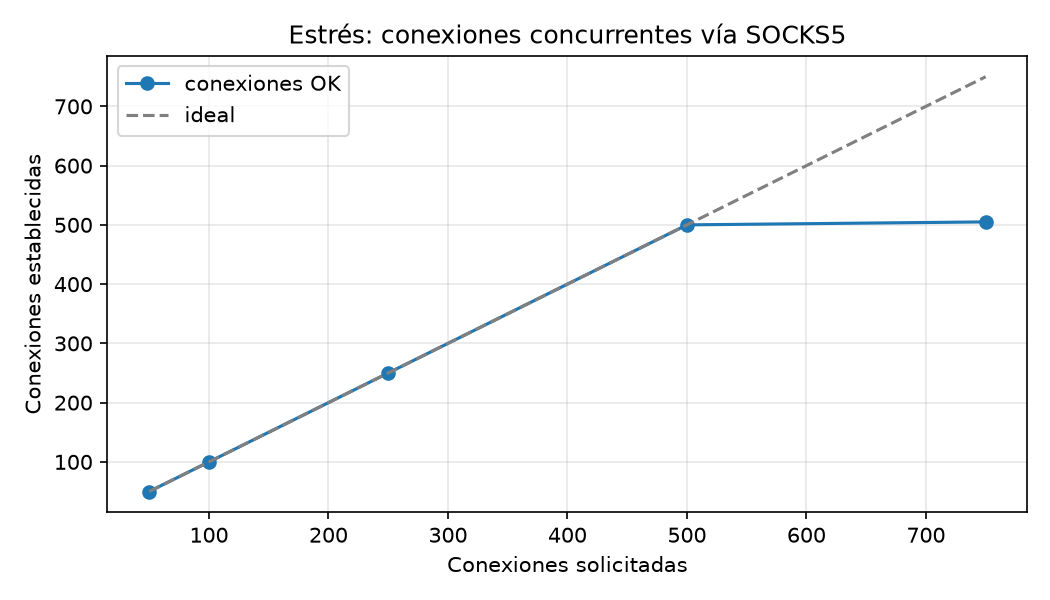
\includegraphics[width=0.85\textwidth]{scripts/results/concurrent.png}
\caption{Conexiones concurrentes solicitadas vs.\ establecidas.}
\end{figure}

\begin{figure}[H]
\centering
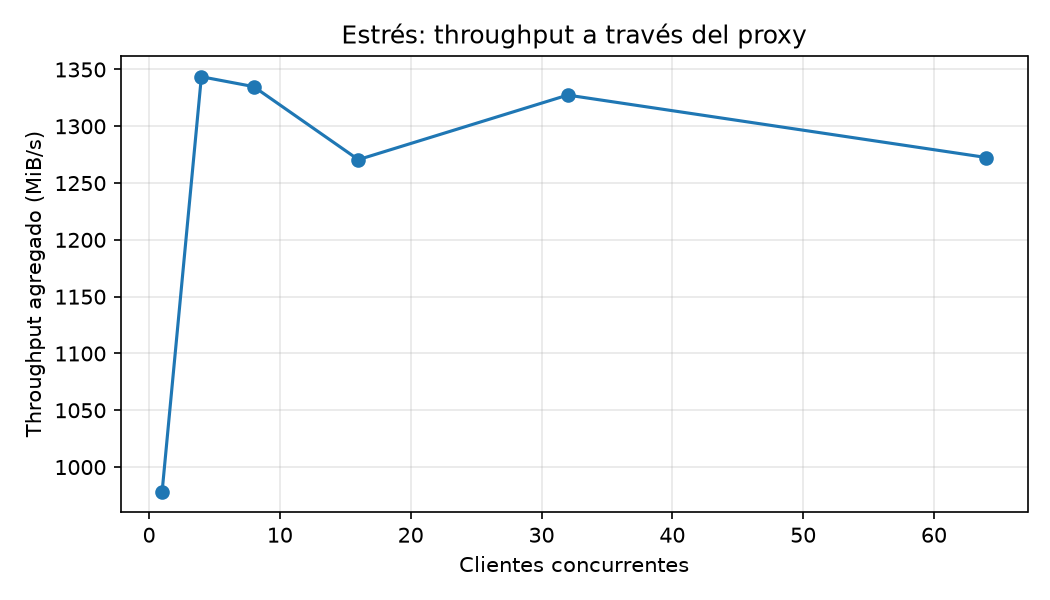
\includegraphics[width=0.85\textwidth]{scripts/results/throughput.png}
\caption{Throughput agregado en loopback (payload 2\,MiB por cliente).}
\end{figure}

En loopback el throughput se mantiene en el orden de cientos/miles de MiB/s y no
es el cuello de botella: la degradación relevante aparece en la cantidad de
conexiones concurrentes, no en el ancho de banda local. Para reproducir:

\begin{lstlisting}[caption=Reproducir estrés]
$ bash scripts/run_stress.sh
\end{lstlisting}

% =============================================================================
\section{Guía de instalación}

\subsection{Requisitos}

\begin{itemize}
    \item Linux con GCC compatible con C11 (o Clang), GNU Make y pthreads.
    \item Python~3 con \texttt{matplotlib} y \texttt{numpy} (opcional, para las pruebas de estrés y gráficos).
    \item \texttt{curl} (opcional, para verificar el proxy manualmente).
\end{itemize}

\subsection{Compilación}

Para compilar el servidor y el cliente:

\begin{lstlisting}[caption=Compilar el proyecto]
$ make clean && make all
\end{lstlisting}

Los artefactos generados son:

\begin{itemize}
    \item \texttt{bin/server} --- servidor proxy SOCKS5.
    \item \texttt{bin/client} --- cliente de monitoreo y configuración.
\end{itemize}

Los objetos intermedios se depositan en \texttt{obj/}. Para limpiar:

\begin{lstlisting}[caption=Limpiar artefactos de compilación]
$ make clean
\end{lstlisting}

\subsection{Verificación rápida}

Una vez compilado, se puede verificar que el servidor arranca correctamente:

\begin{lstlisting}[caption=Verificación de arranque]
$ ./bin/server -A test123
Listening on TCP port 1080
Management listening on TCP port 8080
\end{lstlisting}

Para detenerlo: \texttt{Ctrl+C} (SIGINT) realiza un graceful shutdown.

\subsection{Ejecución de pruebas de estrés (opcional)}

\begin{lstlisting}[caption=Ejecutar harness de estrés]
$ bash scripts/run_stress.sh
\end{lstlisting}

Requiere Python~3 con \texttt{matplotlib} y \texttt{numpy}. Los resultados se guardan en \texttt{scripts/results/}.

% =============================================================================
\section{Instrucciones para la configuración}

\begin{lstlisting}[caption=Opciones del servidor]
./bin/server [OPCIONES]

  -h               Ayuda.
  -l <dirección>   Bind SOCKS (defecto: dual-stack / 0.0.0.0 vía IPv6).
  -L <dirección>   Bind management (defecto: 127.0.0.1).
  -p <puerto>      Puerto SOCKS (defecto: 1080).
  -P <puerto>      Puerto management (defecto: 8080).
  -A <secreto>     Secreto de management (defecto: changeme).
  -u <usr>:<pass>  Usuario inicial (puede repetirse, hasta 10).
  -v               Versión.
\end{lstlisting}

\begin{lstlisting}[caption=Opciones del cliente]
./bin/client [OPCIONES] <comando>

  -L <dirección>   IP management (defecto: 127.0.0.1)
  -P <puerto>      Puerto management (defecto: 8080)
  -A <secreto>     Secreto (defecto: changeme)

  get-metrics | add-user <u> <p> | del-user <u> | set-secret <nuevo>
\end{lstlisting}

Los accesos se imprimen en stdout del servidor; para persistirlos:

\begin{lstlisting}[caption=Redirección de logs a archivo]
$ ./bin/server -A mi_secreto -u admin:admin123 > access.log 2> server.err
\end{lstlisting}

% =============================================================================
\section{Ejemplos de configuración y monitoreo}

\subsection{Escenario 1: cambio de secreto en caliente}

\begin{lstlisting}
$ ./bin/server -A secreto_inicial -u admin:admin123

$ ./bin/client -A secreto_inicial set-secret nuevo_secreto
secreto actualizado

$ ./bin/client -A secreto_inicial get-metrics
error: unauthorized

$ ./bin/client -A nuevo_secreto get-metrics
conexiones activas: 0
conexiones historicas: 0
bytes transferidos: 0
\end{lstlisting}

\subsection{Escenario 2: múltiples usuarios y verificación de error}

\begin{lstlisting}
$ ./bin/client -A changeme add-user alberto pass1
usuario agregado

$ ./bin/client -A changeme add-user beatriz pass2
usuario agregado

$ ./bin/client -A changeme add-user carlos pass3
usuario agregado

$ ./bin/client -A changeme del-user alberto
usuario eliminado

$ ./bin/client -A changeme del-user alberto
error: user not found
\end{lstlisting}

\subsection{Escenario 3: auditoría de accesos}

\begin{lstlisting}
$ ./bin/server -A mi_secreto -u admin:admin123 > access.log
$ cat access.log
[2026-07-12 16:46:17] User: admin | FQDN: example.com | IP Destino: 93.184.216.34:80
\end{lstlisting}

% =============================================================================
\section{Documento de diseño del proyecto}

\subsection{Diagrama de módulos}

\begin{verbatim}
+------------------------------------------------------------------+
|                        bin/server                                 |
|  main.c / args.c     socks5nio.c (STM SOCKS5 + COPY)              |
|  hello.c / auth.c / request.c   mng_server.c (STM management)     |
|  [infra: selector, buffer, stm, netutils]                         |
+------------------------------------------------------------------+
|                        bin/client                                 |
|  client.c  -- CLI: parsea +OK/-ERR, salida humana                 |
+------------------------------------------------------------------+
\end{verbatim}

La infraestructura de multiplexación (\texttt{selector}, \texttt{buffer},
\texttt{stm}) se reutiliza como base; el aporte propio está en el proxy SOCKS5
(\texttt{socks5nio} y parsers), el protocolo de management y el cliente CLI.

\subsection{Componentes propios}

\subsubsection{Máquina de estados SOCKS5 (\texttt{socks5nio.c})}

Implementa el ciclo de vida completo de cada conexión: HELLO, AUTH, REQUEST
(resolución + connect no bloqueante), respuesta REP y túnel COPY con write
optimista y propagación de \texttt{shutdown} parciales.

\subsubsection{Parsers SOCKS5}

\begin{itemize}
    \item \texttt{hello.c/h}: oferta y selección de métodos.
    \item \texttt{auth.c/h}: usuario/contraseña RFC~1929.
    \item \texttt{request.c/h}: CONNECT con IPv4, IPv6 y FQDN; marshalling de REP.
\end{itemize}

\subsubsection{Servidor de monitoreo (\texttt{mng\_server.c})}

STM propia (\texttt{MNG\_READ $\rightarrow$ MNG\_EXECUTE $\rightarrow$ MNG\_WRITE})
sobre el mismo selector. Autentica por secreto, muta la tabla de usuarios y expone
métricas.

\subsubsection{Cliente de monitoreo (\texttt{client.c})}

Abstrae el protocolo: no es un netcat. Traduce subcomandos POSIX a líneas del
protocolo y presenta resultados legibles con códigos de salida útiles para scripts.

\subsection{Flujo de una conexión SOCKS5}

\begin{verbatim}
Cliente SOCKS5              Servidor Proxy              Servidor Origen
      |--- HELLO ----------------->|                            |
      |<-- METHOD -----------------|                            |
      |--- AUTH (opcional) ------->|                            |
      |<-- STATUS -----------------|                            |
      |--- REQUEST CONNECT ------->|                            |
      |                            |======= CONNECT ===========>|
      |<-- REP --------------------|                            |
      |=========== TÚNEL BIDIRECCIONAL (COPY) =================>|
\end{verbatim}

\end{document}
